\section{Performance Evaluation}\label{sec:exp}

We evaluate \dualtree and its pruning variants on fully dynamic high-dimensional kNN join workloads. The experiments are designed to answer three questions: whether the dual-index architecture improves over one-sided dynamic baselines, whether fine-grained pruning adds measurable benefit beyond the base architecture, and whether the proposed dimensionality-selection models choose near-optimal pruning dimensions.

\subsection{Experimental Setup}

\noindent\textbf{Methods.}
We compare the following methods.

\begin{itemize}
    \item \textbf{\dualtree}: the proposed dual-index framework without the leaf-level fine-grained pruning stage.
    \item \textbf{\dualtreeopt}: \dualtree with fine-grained pruning, using the mixture-model dimensionality selection from Section~\ref{sec:pruning}.
    \item \textbf{\dualtreefast}: \dualtree with fine-grained pruning, using the simplified log-linear dimensionality selection from Equation~\ref{equ:simppd}.
    \item \textbf{Scan}: recomputes the affected join results by brute force after each update.
    \item \textbf{iDistance}~\cite{jagadish2005idistance}: an adapted high-dimensional index baseline for workloads where the query side is updated.
    \item \textbf{Spheretree}~\cite{yang2014continuous}: an adapted baseline for workloads where the reference side is updated.
    \item \textbf{\hdrtree}~\cite{ukey2022efficient}: an ablation that indexes only $U$; forward kNN search over $I$ is not accelerated.
    \item \textbf{\deltatree}~\cite{cui2003contorting}: an ablation that indexes only $I$; reverse kNN search over $U$ is not accelerated.
\end{itemize}

All evaluated methods return exact kNN join results. We therefore do not compare against approximate nearest-neighbor methods, whose recall-quality trade-offs are orthogonal to the exact maintenance problem studied here.

\noindent\textbf{Datasets and hardware.}
Table~\ref{tab:dataset} summarizes the eight real datasets used in the evaluation. They cover image, audio, and text features, with dimensionalities from 128 to 4096. All experiments were run on a server with two Intel Xeon Gold 6342 CPUs, 500 GB RAM, and Ubuntu 22.04.1 LTS.

\begin{table}[t]
\centering
\caption{Dataset summary.}
\label{tab:dataset}
\begin{tabular}{@{}lrrl@{}}
\toprule
\textbf{Dataset} & \textbf{Records} & \textbf{Dims} & \textbf{Type}\\
\midrule
NUS-WIDE & 260,000 & 128 & Image\\
Fashion-MNIST & 60,000 & 784 & Image\\
Audio & 53,000 & 192 & Audio\\
Cifar & 50,000 & 512 & Image\\
Trevi & 100,000 & 4096 & Image\\
Sun & 79,000 & 512 & Image\\
Enron & 95,000 & 1369 & Text\\
Millionsong & 1,000,000 & 420 & Audio\\
\bottomrule
\end{tabular}
\end{table}

\noindent\textbf{Evaluation protocol.}
The main parameter study uses NUS-WIDE, a standard high-dimensional benchmark dataset~\cite{hussain2024gradual}. The mixed workload contains insertions into $U$, insertions into $I$, and deletions from $I$. Deletions from $U$ are omitted because they require only removing the corresponding row from the maintained join table. We then isolate the three update types to explain the mixed-workload results, test generality across the other seven datasets, and validate the cost model by comparing predicted pruning dimensions against empirically optimal dimensions.

\subsection{Core Performance on NUS-WIDE}

\noindent\textbf{Parameter sensitivity under mixed updates.}
Figure~\ref{fig:main-figure-4-plots} reports the effect of update count, initial set size, and $k$ under mixed updates. In Figure~\ref{fig:sub-a}, total time increases with the number of updates because every insertion or deletion triggers kNN search, RkNN search, or repair operations. The proposed pruning variants consistently improve over the base \dualtree: \dualtreefast is 28.4\% to 35.6\% faster than \dualtree, while \dualtreeopt adds another 8.7\% to 9.1\% improvement.

The same pattern holds when varying the initial set size in Figure~\ref{fig:sub-b}. Larger sets expand both the forward and reverse search spaces, increasing the cost for all methods. Even so, the dual-index architecture remains effective: \dualtree is up to 23\% faster than the strongest one-sided baseline, \deltatree, and the two pruning variants provide further reductions.

Figure~\ref{fig:sub-c} varies the number of neighbors. Larger $k$ values increase pruning bounds and make both kNN and RkNN searches less selective. \dualtreefast remains 28.2\% to 36.9\% faster than \dualtree, and \dualtreeopt improves on \dualtreefast by another 9.2\% to 9.7\%. The results show that both the architecture and the pruning model remain stable as the join output size grows.

\begin{figure*}[t]
    \centering
    \begin{subfigure}[b]{0.48\textwidth}
        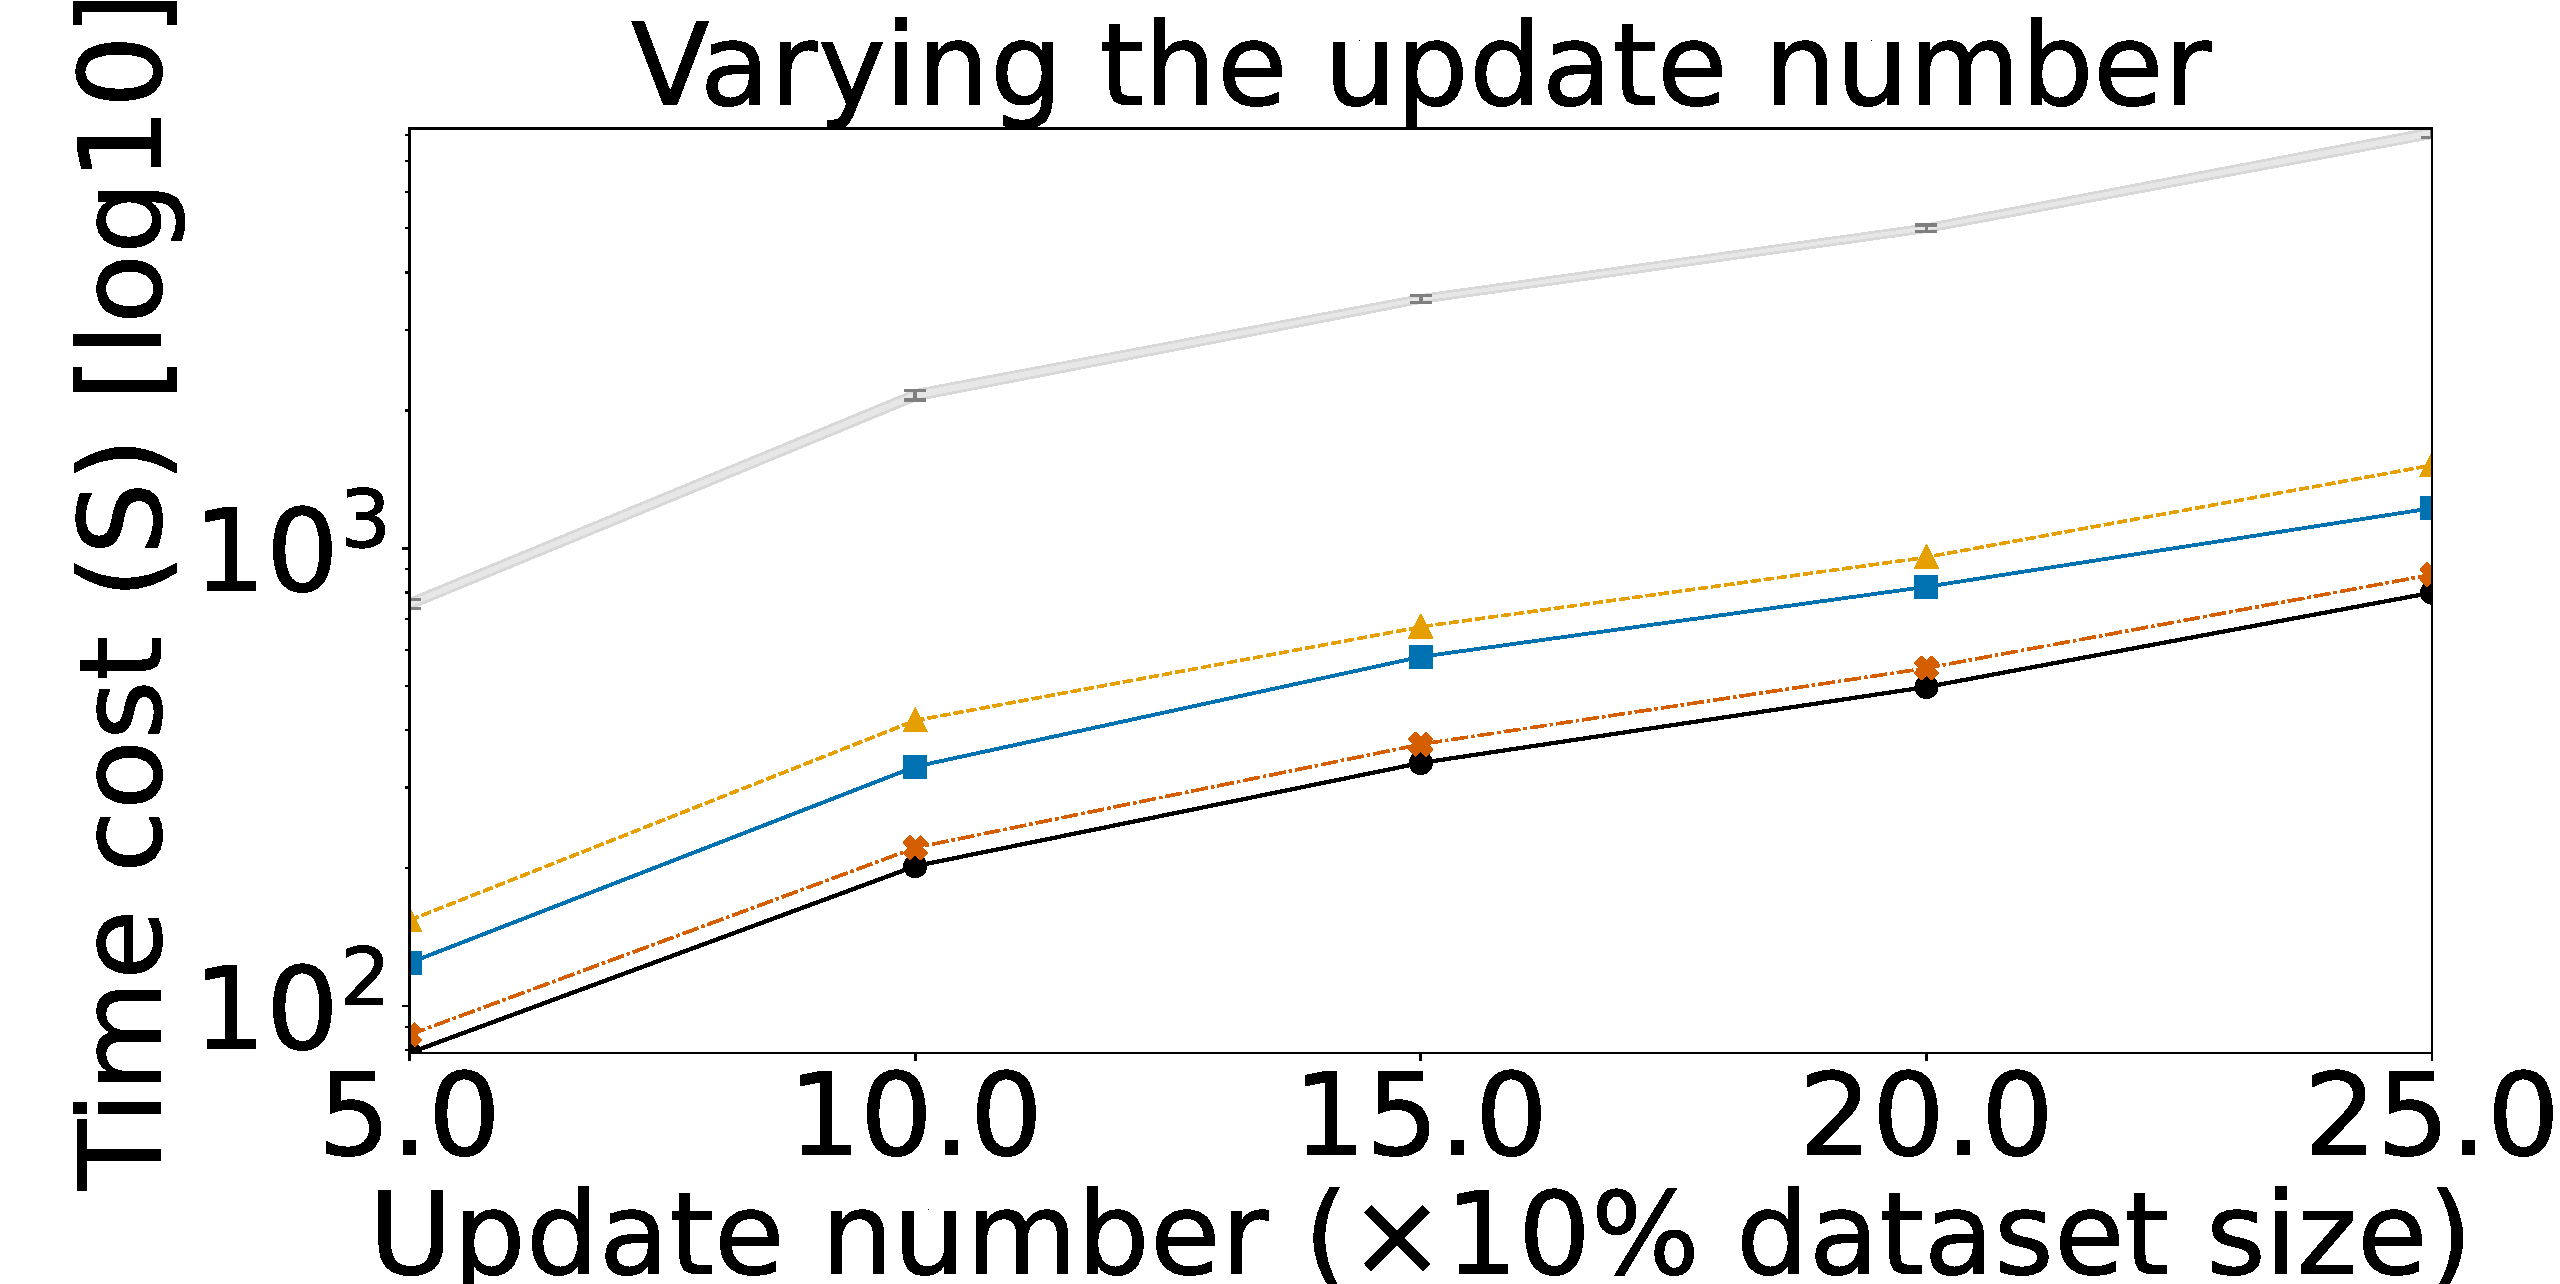
\includegraphics[width=\linewidth]{Images/realgraph/Varying the update number.pdf}
        \caption{Time vs. number of updates.}
        \label{fig:sub-a}
    \end{subfigure}
    \hfill
    \begin{subfigure}[b]{0.48\textwidth}
        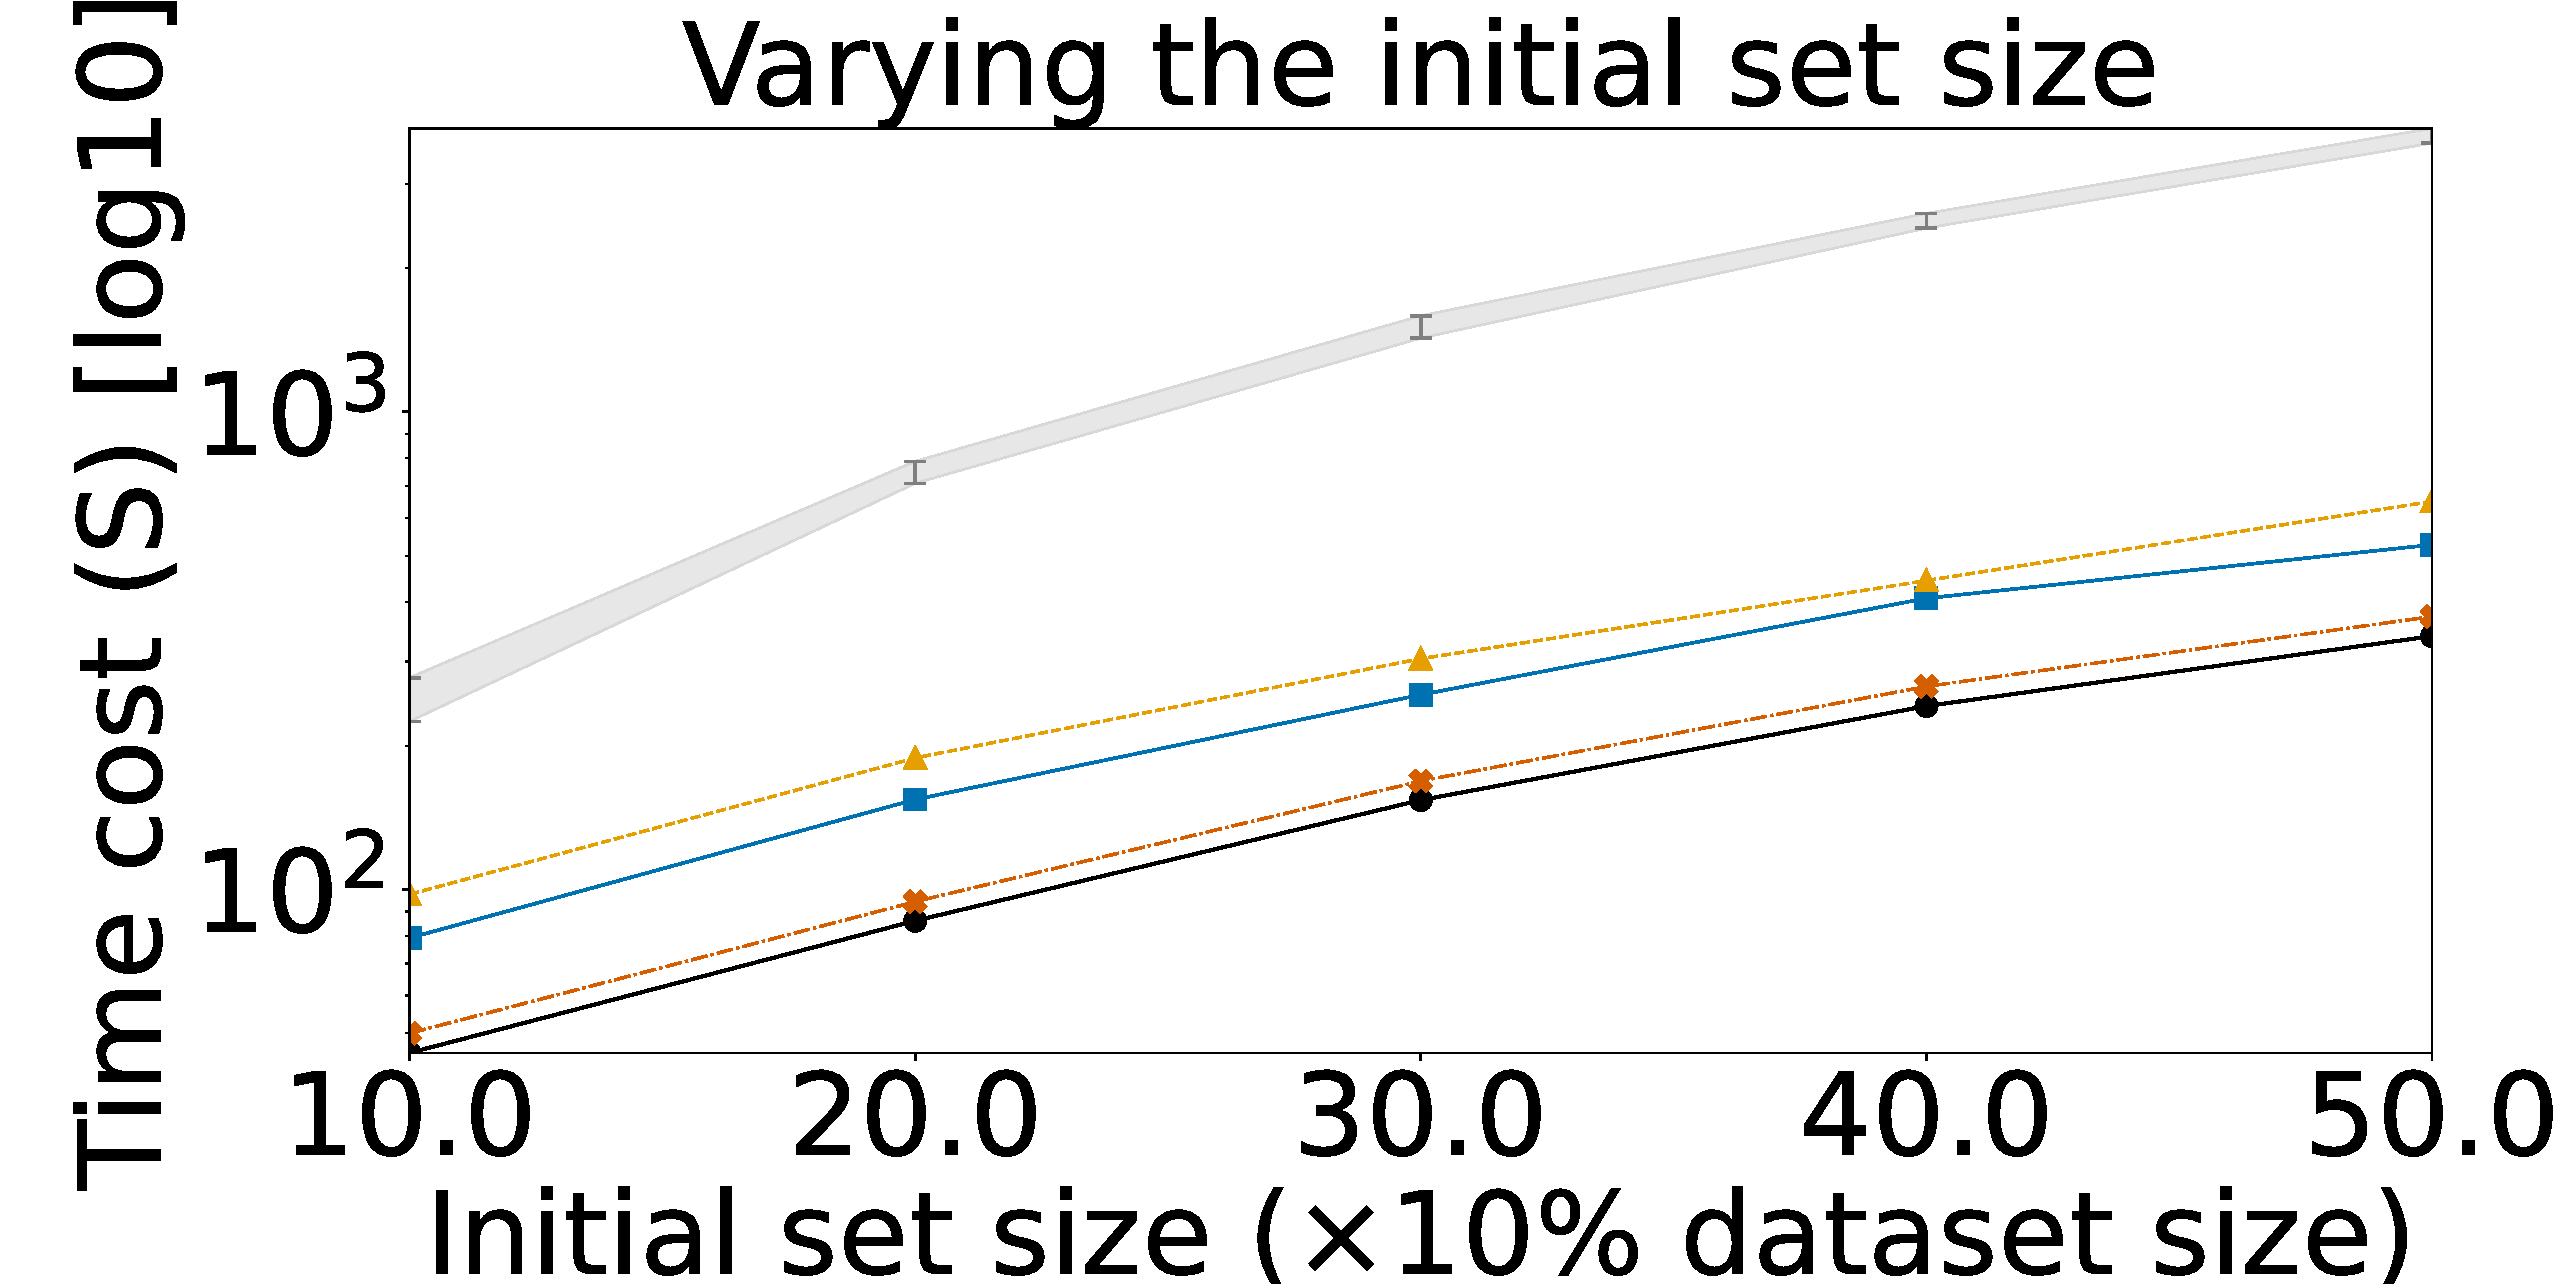
\includegraphics[width=\linewidth]{Images/realgraph/vary_initial_set_size_real_pdf.pdf}
        \caption{Time vs. initial set size.}
        \label{fig:sub-b}
    \end{subfigure}

    \vspace{0.8em}

    \begin{subfigure}[b]{0.48\textwidth}
        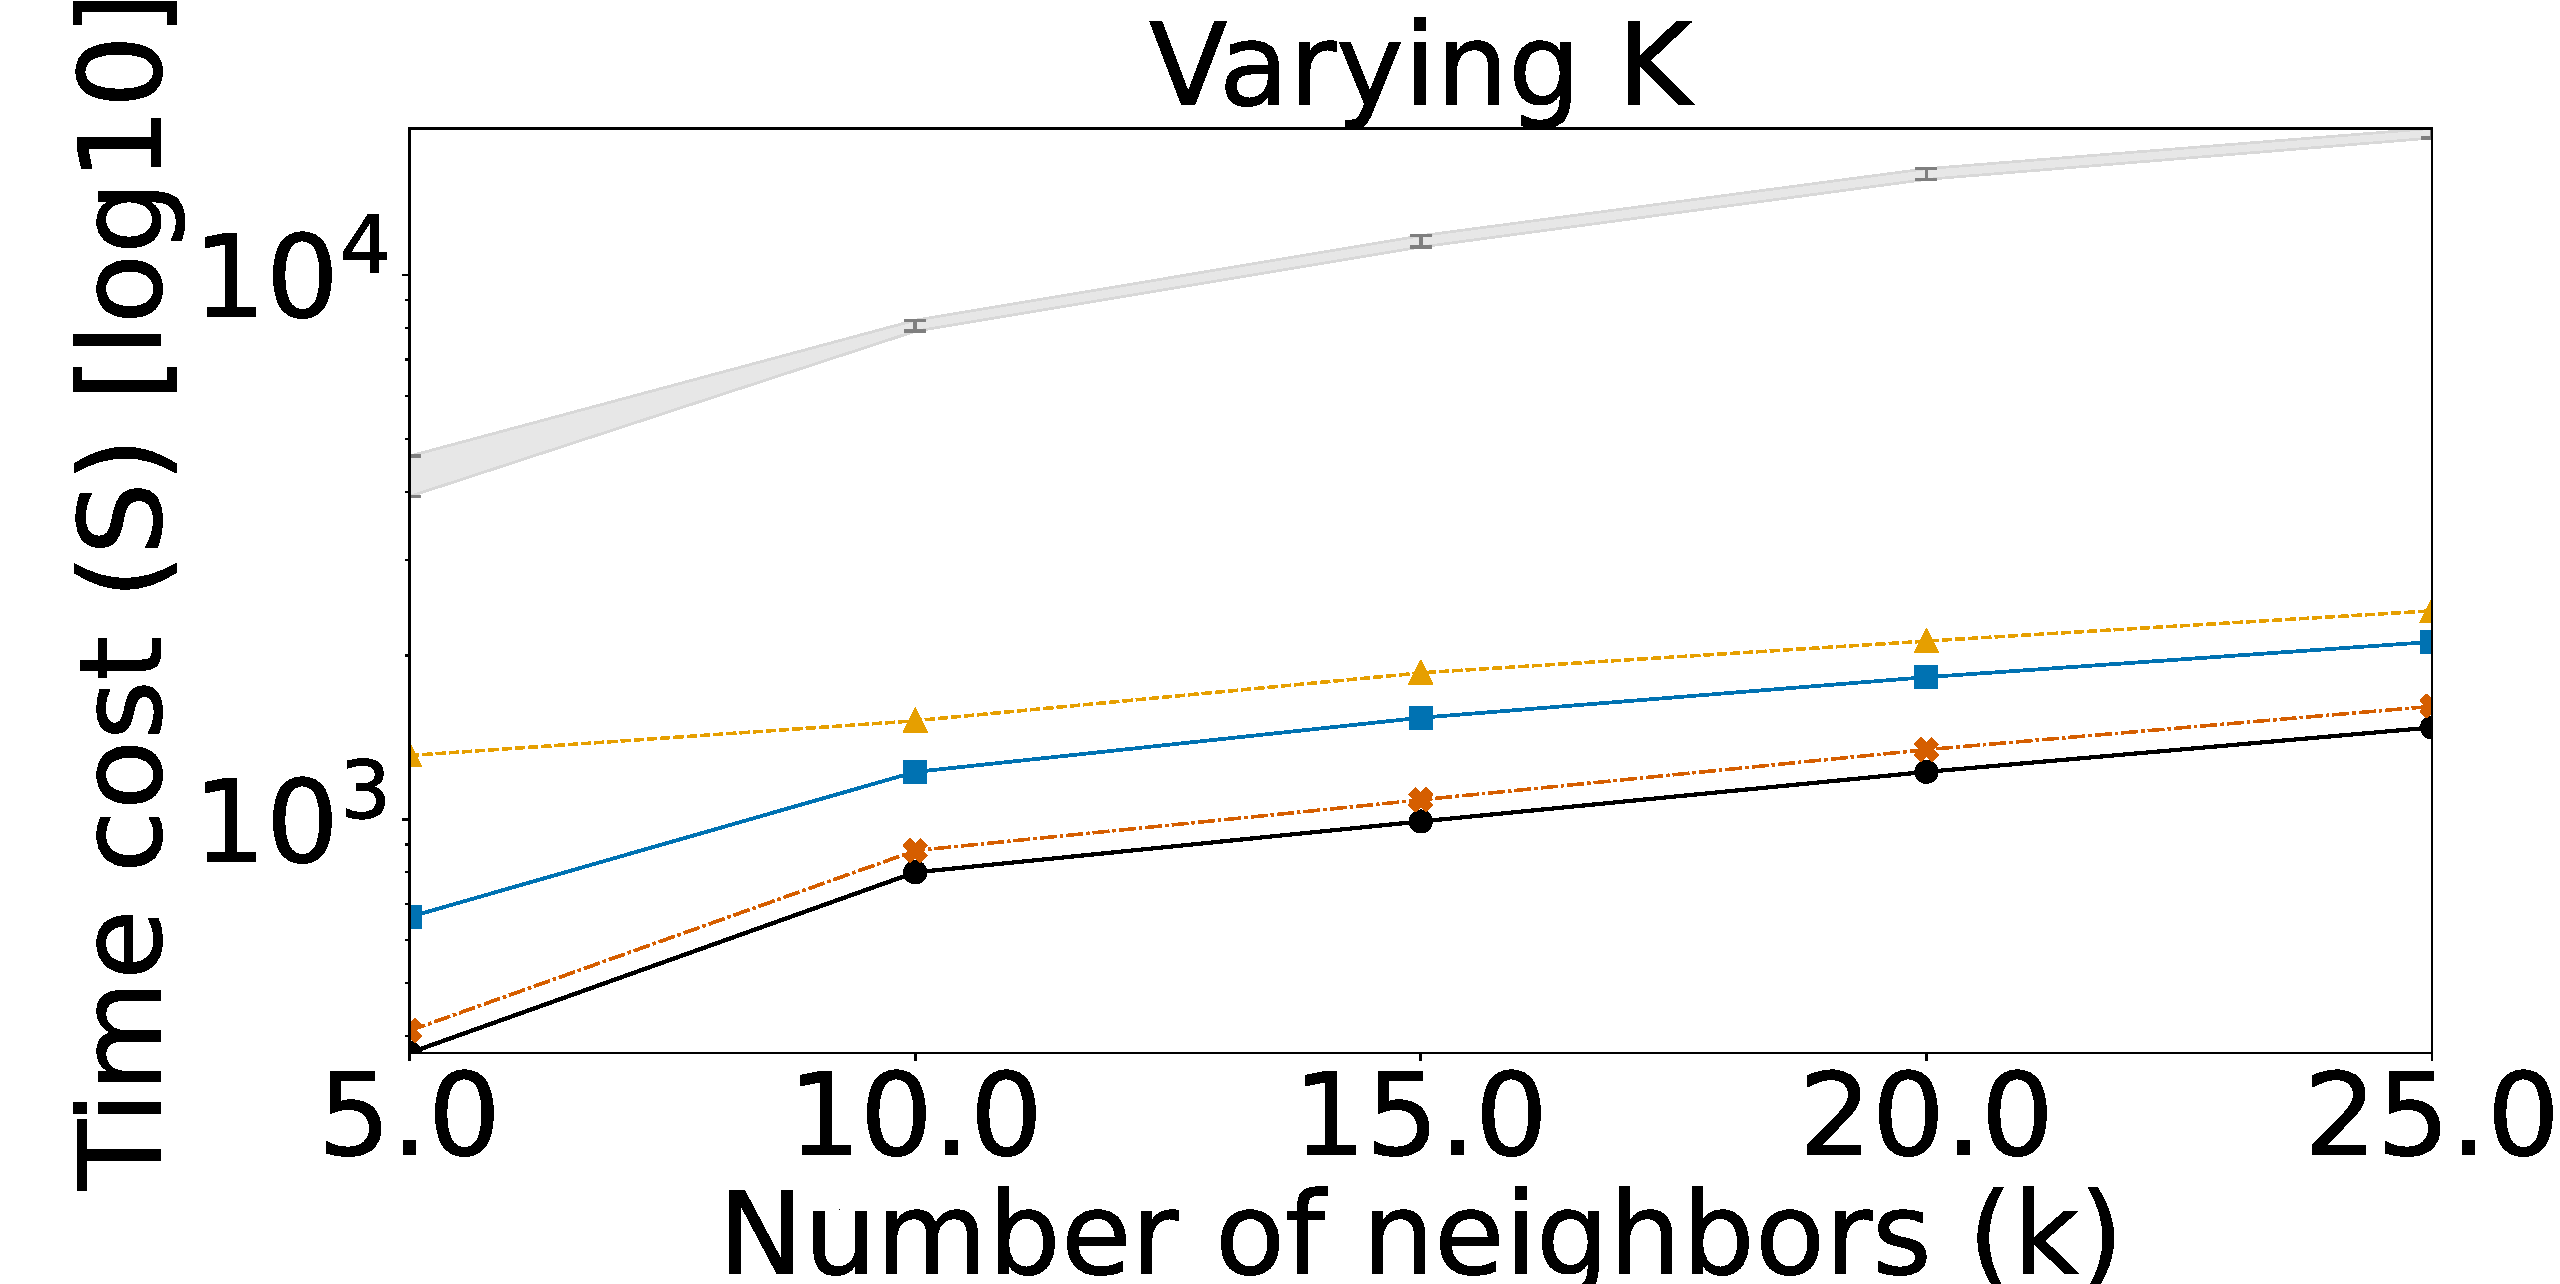
\includegraphics[width=\linewidth]{Images/realgraph/vary_k_real_pdf.pdf}
        \caption{Time vs. number of neighbors.}
        \label{fig:sub-c}
    \end{subfigure}
    \hfill
    \begin{subfigure}[b]{0.48\textwidth}
        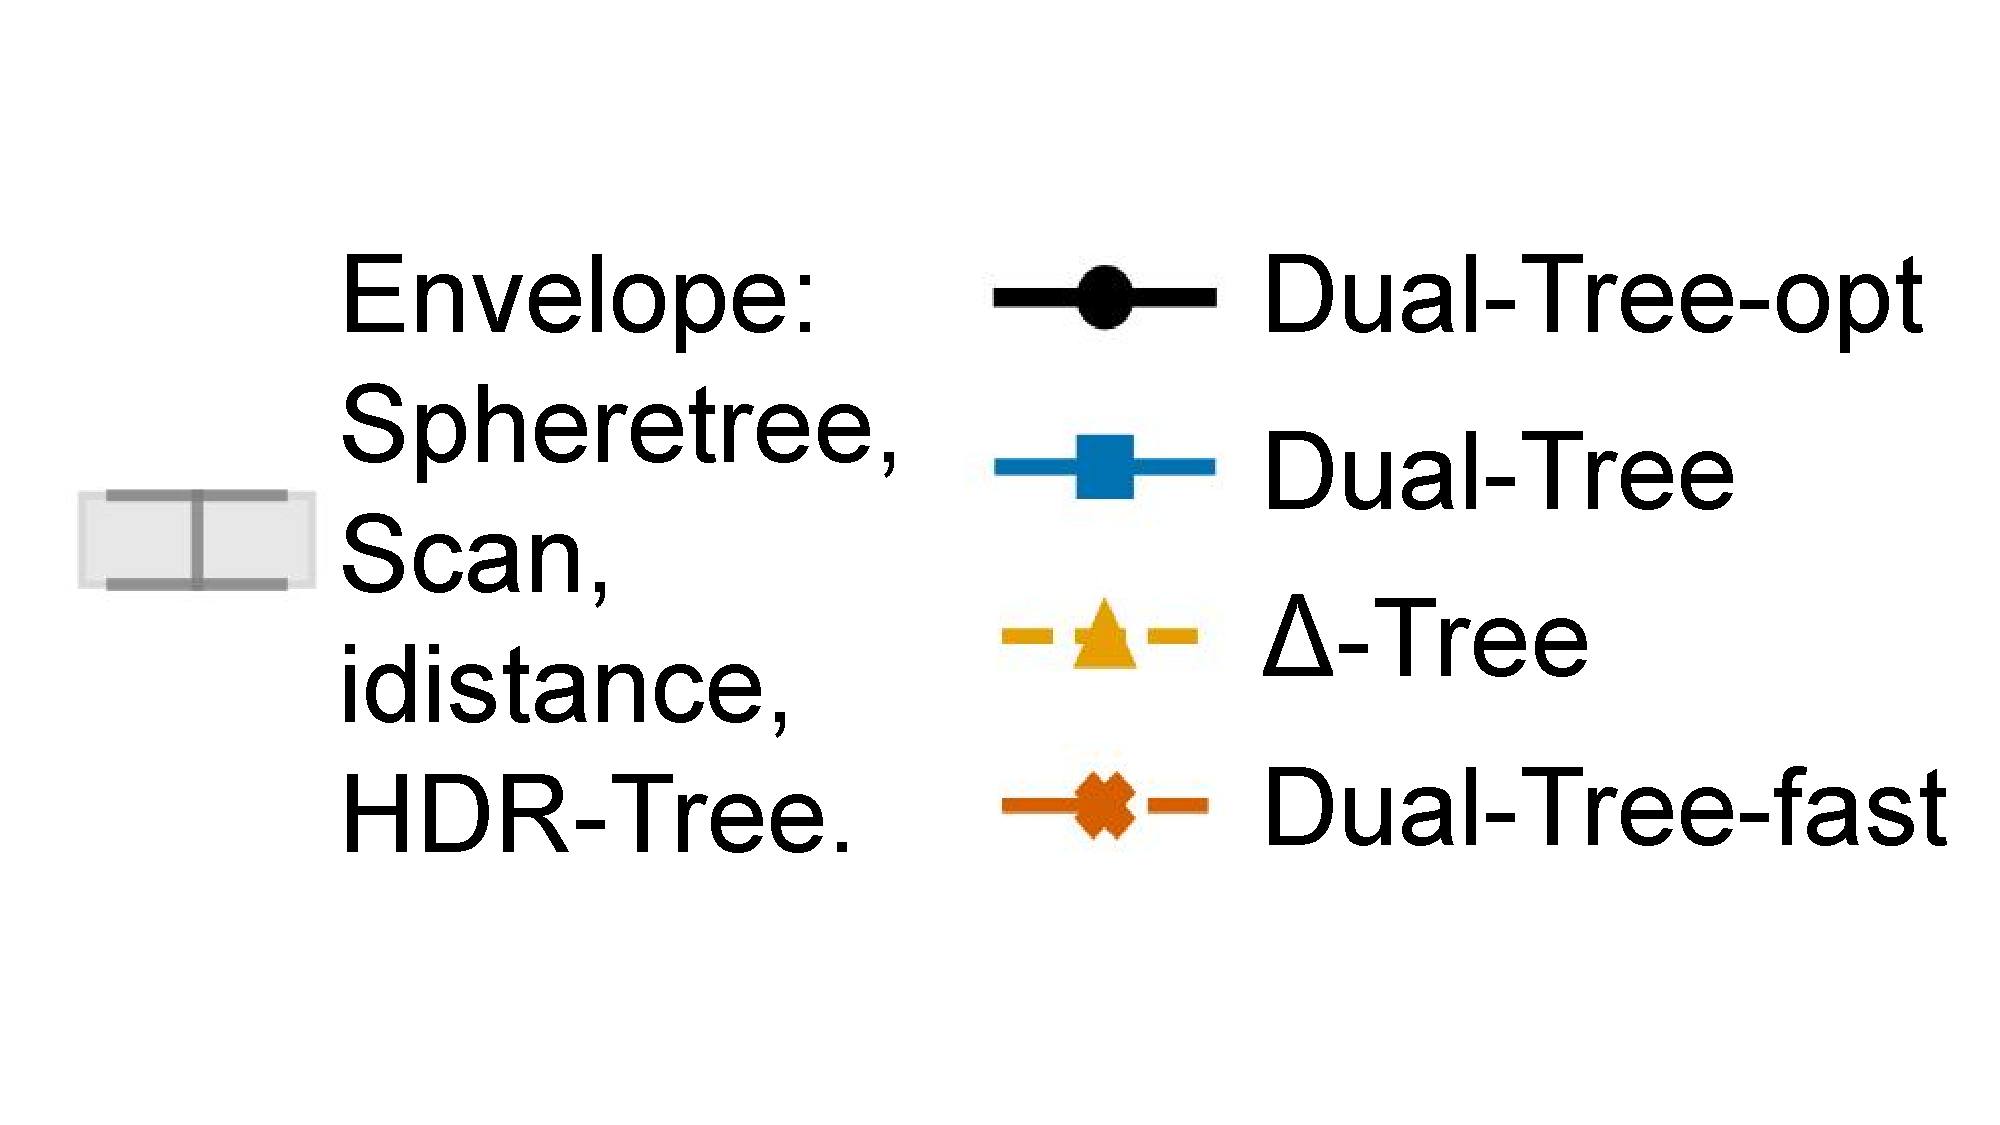
\includegraphics[width=\linewidth]{Images/realgraph/legende.pdf_2.pdf}
        \caption{Legend.}
        \label{fig:subd}
    \end{subfigure}

    \caption{Parameter sensitivity on the NUS-WIDE mixed workload.}
    \label{fig:main-figure-4-plots}
\end{figure*}

\noindent\textbf{Single update types.}
Table~\ref{tab:single-update-performance} isolates the three update types. Deleting from $I$ is the most expensive case because it requires locating affected queries by RkNN search and then repairing their kNN lists. This workload exposes the weakness of one-sided indexes. \dualtree is over 8.2$\times$ faster than \hdrtree and 1.2$\times$ faster than \deltatree because it accelerates both primitives. The pruning variants are also strong on the workloads where one-sided indexes are specialized: \dualtreeopt is 1.9$\times$ faster than \deltatree on insertions into $U$ and 1.3$\times$ faster than \hdrtree on insertions into $I$.

\begin{table}[t]
\centering
\caption{Performance in seconds on single update types on NUS-WIDE. The size of the non-updated set is fixed at $S/2$, where $S$ is the dataset size.}
\label{tab:single-update-performance}
\begin{tabular}{@{}lrrr@{}}
\toprule
\textbf{Method} & \textbf{$U$ ins.} & \textbf{$I$ ins.} & \textbf{$I$ del.} \\
\midrule
\dualtreeopt    & 49   & 263  & 498   \\
\dualtreefast   & 54   & 275  & 545   \\
\dualtree       & 96   & 370  & 785   \\
\midrule
\deltatree      & 95   & 500  & 952   \\
\hdrtree        & 884  & 360  & 6469  \\
iDistance       & 798  & 507  & 7127  \\
Spheretree      & 890  & 406  & 7300  \\
Linear Scan     & 881  & 497  & 7355  \\
\bottomrule
\end{tabular}
\end{table}

\subsection{Generality Across Datasets}

Table~\ref{tab:generality-results} reports mixed-workload performance on the other seven datasets. The initial set size and the number of updates are both set to 25\% of the dataset size, and $k$ is fixed to 10. \dualtreeopt is the fastest method on every dataset. The base \dualtree already outperforms the strongest one-sided baseline, \deltatree, with speedups from 1.06$\times$ on Audio to 1.47$\times$ on Fashion-MNIST. After adding fine-grained pruning, \dualtreeopt achieves an average speedup of 1.88$\times$ over \deltatree. The largest gain occurs on Trevi, where the 4096-dimensional feature space makes full-dimensional verification especially expensive and \dualtreeopt is 2.65$\times$ faster than \deltatree.

\begin{table*}[t]
\centering
\caption{Performance in seconds on the mixed workload across seven additional datasets. Best results are in bold.}
\label{tab:generality-results}
\setlength{\tabcolsep}{5pt}
\begin{tabular}{@{}lrrrrrrr@{}}
\toprule
\textbf{Method} & \textbf{Cifar} & \textbf{Audio} & \textbf{Msong} & \textbf{Sun} & \textbf{Trevi} & \textbf{MNIST} & \textbf{Enron} \\
\midrule
\dualtreeopt    & \textbf{500} & \textbf{100} & \textbf{3373} & \textbf{626} & \textbf{3716} & \textbf{244} & \textbf{3687} \\
\dualtreefast   & 524 & 115 & 3453 & 672 & 4076 & 268 & 3799 \\
\dualtree       & 700 & 170 & 5159 & 945 & 6944 & 371 & 4786 \\
\midrule
\deltatree      & 785 & 181 & 5606 & 1123 & 9851 & 545 & 5387 \\
\hdrtree        & 900 & 358 & 15288 & 2475 & 19482 & 1612 & 7473 \\
iDistance       & 862 & 275 & 14155 & 1883 & 17326 & 1120 & 6338 \\
Spheretree      & 912 & 367 & 15997 & 2485 & 21166 & 1694 & 7959 \\
Linear Scan     & 978 & 378 & 16044 & 2422 & 22866 & 1789 & 8255 \\
\bottomrule
\end{tabular}
\end{table*}

\subsection{Validation of the Cost Model}

\noindent\textbf{Cost-dimensionality curve.}
Figure~\ref{fig:main-figure-two-plots} plots the leaf-level processing time on Trevi while varying the pruning dimensionality. Both the RkNN-dominant workload and the kNN-dominant workload exhibit a U-shaped curve. At small $d$, adding principal components sharply improves pruning power because the leading components capture most of the variance. After the informative components are exhausted, the marginal pruning gain diminishes and the linear cost of the low-dimensional check dominates.

\begin{figure*}[t]
    \centering
    \begin{subfigure}[b]{0.48\textwidth}
        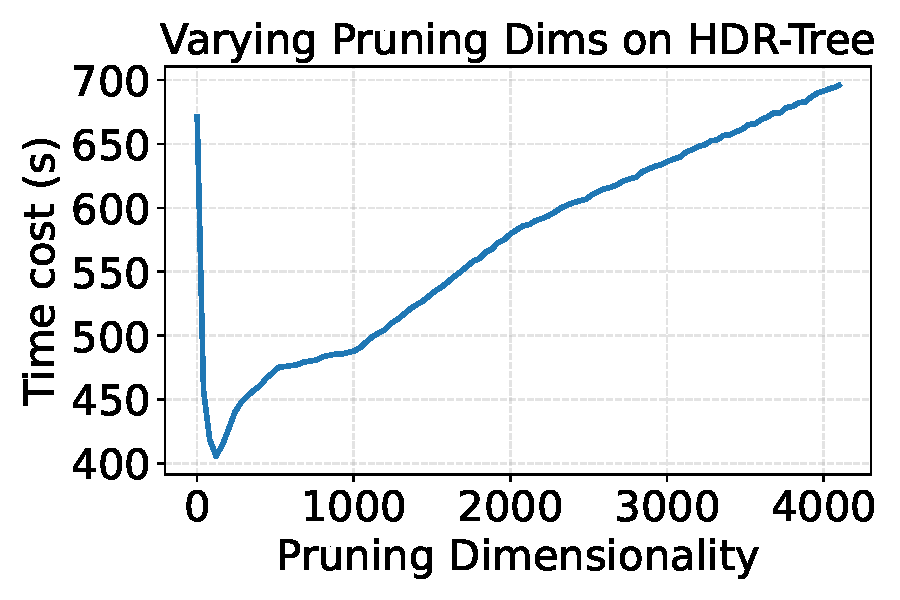
\includegraphics[width=\linewidth]{Images/realgraph/dim_hdr_pdf.pdf}
        \caption{RkNN workload.}
        \label{fig:sub-a_1}
    \end{subfigure}
    \hfill
    \begin{subfigure}[b]{0.48\textwidth}
        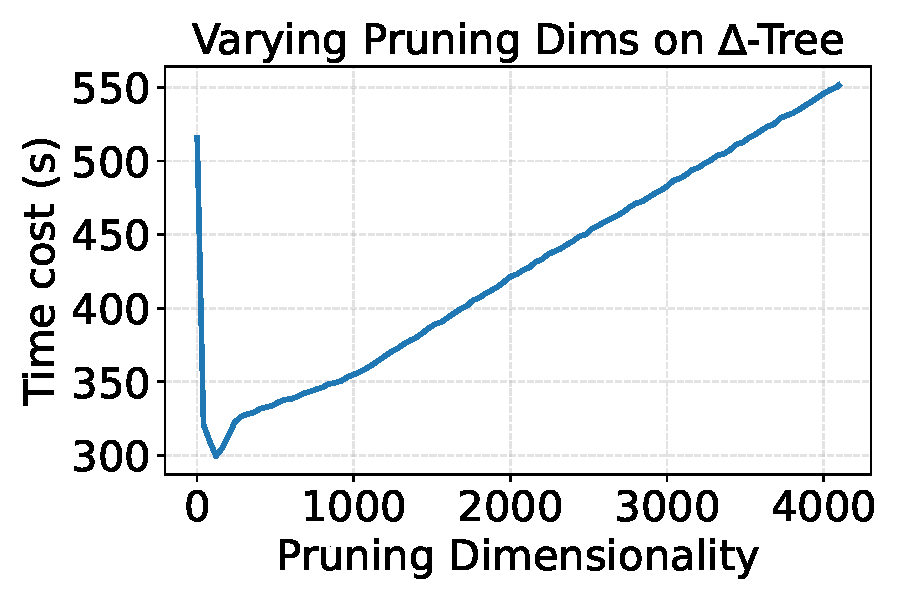
\includegraphics[width=\linewidth]{Images/realgraph/dim_delta_pdf.pdf}
        \caption{kNN workload.}
        \label{fig:sub-b_1}
    \end{subfigure}
    \caption{Leaf-level cost as a function of pruning dimensionality.}
    \label{fig:main-figure-two-plots}
\end{figure*}

\noindent\textbf{Prediction accuracy.}
Table~\ref{tab:model-validation} compares the dimensions predicted by \dualtreeopt and \dualtreefast with the empirically best dimension on all eight datasets. Each cell reports dimensional error and the corresponding execution-time error. \dualtreeopt keeps time error below 4\% in almost all cases and reaches 0\% error on Enron. \dualtreefast has larger dimensional error because it uses only a two-point log-linear fit, but its time error is still small in most cases. This confirms that the expected-cost model identifies dimensions near the flat bottom of the U-shaped cost curve, where small dimensional deviations cause limited performance loss.

\begin{table}[t]
\centering
\caption{Validation of the cost model on eight datasets. Each cell reports \textbf{dimension/time} error in percent.}
\label{tab:model-validation}
\begin{tabularx}{\columnwidth}{@{}l *{4}{>{\centering\arraybackslash}X}@{}}
\toprule
& \multicolumn{2}{c}{\textbf{RkNN on \hdrtree}} & \multicolumn{2}{c}{\textbf{kNN on \deltatree}} \\
\cmidrule(lr){2-3}\cmidrule(lr){4-5}
\textbf{Dataset} & \makecell{opt \\ Dim/Time} & \makecell{fast \\ Dim/Time} & \makecell{opt \\ Dim/Time} & \makecell{fast \\ Dim/Time} \\
\midrule
NUS-WIDE    & 13.9/1.1 & 14.7/1.4 & 18.5/2.3 & 23.3/2.9 \\
Cifar       & 15.3/1.8 & 18.4/2.2 & 12.8/0.4 & 15.1/0.5 \\
Sun         & 10.8/3.4 & 11.8/3.7 & 20.7/4.0 & 26.7/5.2 \\
Audio       & 25.7/2.7 & 28.8/2.5 & 25.7/0.7 & 27.7/0.6 \\
Enron       & 0.0/0.0  & 38.9/4.7 & 0.0/0.0  & 29.5/2.8 \\
MNIST       & 15.6/1.1 & 18.7/1.4 & 25.3/0.0 & 28.3/9.7 \\
Trevi       & 7.9/1.3  & 8.9/1.3  & 8.4/0.8  & 9.2/0.8  \\
Millionsong & 9.5/2.5  & 5.8/3.1  & 10.2/1.2 & 10.4/1.4 \\
\bottomrule
\end{tabularx}
\end{table}
